%!TEX root = ../thesis.tex
\chapter{Introduction}
\label{ch:introduction}

%\epigraph{``As buds give rise by growth to fresh buds, and these, if vigorous, branch out and overtop on all sides many a feebler branch, so by generation I believe it has been with the great Tree of Life, which fills with its dead and broken branches the crust of the earth, and covers the surface with its ever-branching and beautiful ramifications.''}{Charles Darwin, 1872}

\emph{On the Origin of Species} contains a single figure, depicting the ancestry of species as a branching genealogical tree \cite{Darwin:1859uh} (see Figure \ref{fig:darwin_origin}).
Since then, the tree structure has been the dominant framework to understand, visualize, and communicate discoveries about evolution.
Indeed, a primary focus of evolutionary biology has been to expand and fill the \emph{universal tree of life}, the set of evolutionary relationships among all extant organisms on Earth \cite{Bowler:2003uz}.
Traditionally, this was the realm of phenotype-derived taxonomies \kje{[cite]}.
With the advent of molecular data and computational approaches for tree-inference, evolutionary biology has become a bona fide quantitative discipline.
Molecular phylogenetics --- tree building --- has become the standard tool for inferring evolutionary relationships.
Yet a tree is only accurate if the Darwinian model of descent with modification via reproduction is the sole process driving evolution.
However, it has long been recognized that there exist alterative evolutionary processes that allow organisms to exchange genetic material through means beyond simple reproduction.
Notable examples include species hybridization, horizontal gene transfer in bacteria, and meiotic recombination in eukaryotes.
Collectively, these processes are known as \emph{horizontal evolution}, in contrast to descent with modification, an example of \emph{vertical evolution}.
Increasing genomic data, powered by new high-throughput sequencing technologies, has shown that these horizontal processes are much more prevalent than previously believed.
For some, this has called into question the tree of life hypothesis as an organizing principle and prompted the search for new ways of representing evolutionary relationships \cite{Doolittle:1999,OMalley:2011tu}.

The aim of this thesis is to present a new ways of quantifying and representing nonvertical evolutionary processes using recently developed tools from algebraic and computational topology.
These tools fall under the collective heading of \emph{topological data analysis}, a new branch of applied topology concerned with inferring structure in high-dimensional data sets.
In the following brief introduction, we survey salient aspects of molecular evolution, the tree paradigm, and the challenges therein.
We then introduce the idea of representing evolution as a topological space and give a flavor of our results.

\begin{figure}
\centering
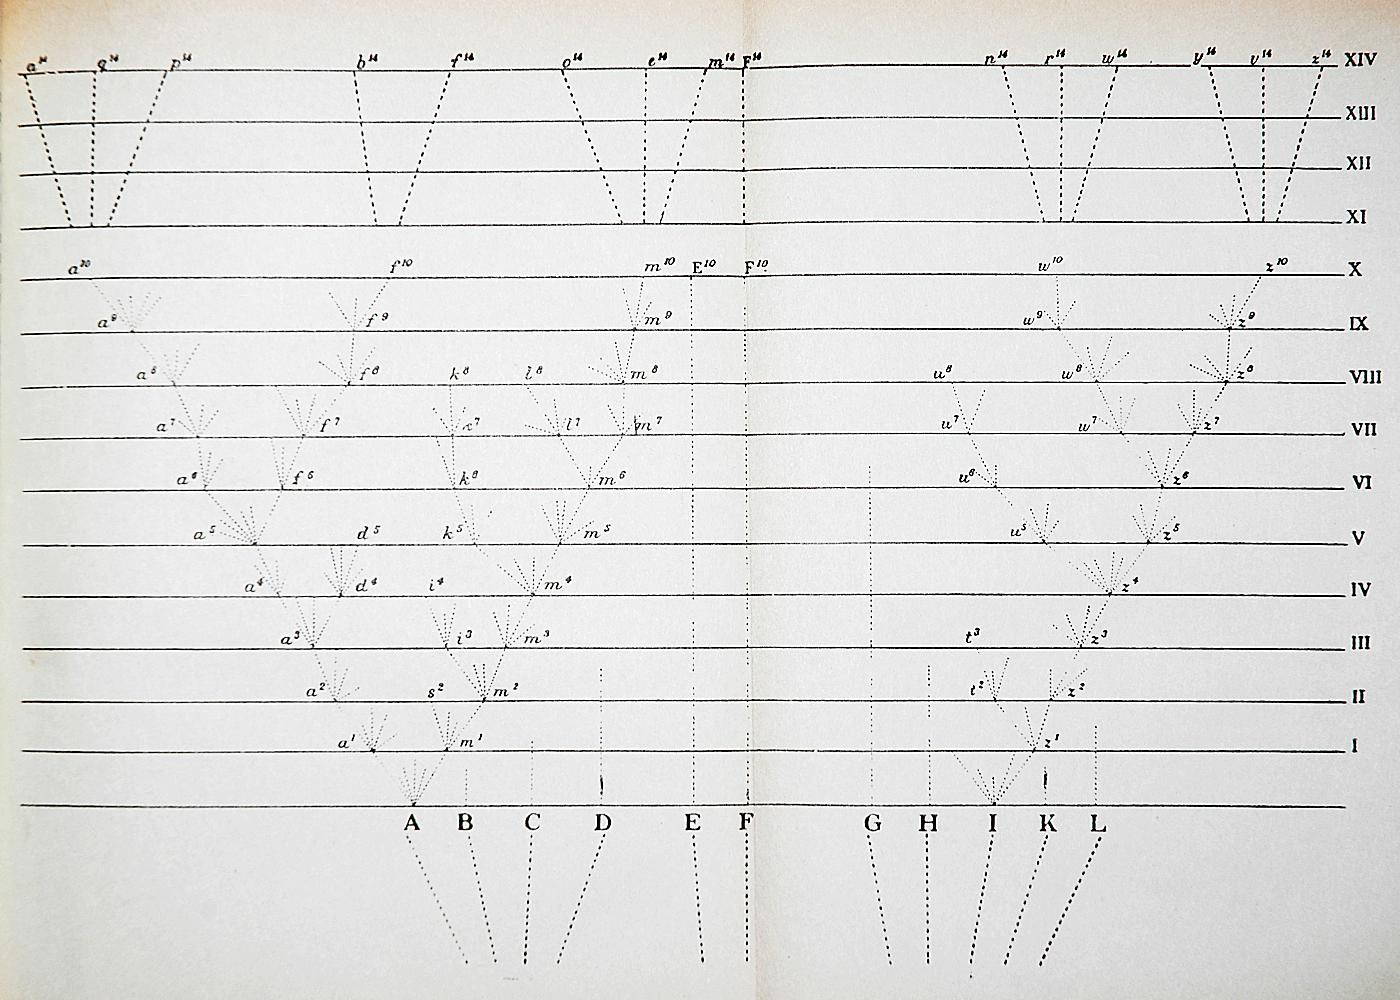
\includegraphics[width=.75\columnwidth]{./fig/introduction/Darwin_divergence.jpg}
\caption[Charles Darwin's Tree]{The only figure in Darwin's Origin of Species.}
\label{fig:darwin_origin}
\end{figure}

\section{Molecular Evolution and the Tree Paradigm}

The combination of Darwin's ideas of natural selection with Mendelian genetics led to the \emph{modern evolutionary synthesis}, outlined in the first half of the twentieth century in pioneering works by Fisher, Wright, Haldane, and others (see \cite{Huxley:1942} and \cite{Gould:2002ts} for historical detail).
The synthesis was based largely on analysis of distributions of allele frequencies in distinct populations, the purview of classical population genetics.
The field was placed on molecular foundations with the Watson and Crick's discovery of the DNA double-helix in 1953 \cite{Watson:1953wm}.
These developments led to the modern study of \emph{molecular evolution}, the analysis of how processes such as mutation, drift, and recombination act at the cellular level to induce changes in populations and species.
While molecular biology has focused on the biochemical and biophysial mechanisms underlying these processes, \emph{molecular phylogenetics} has focused on the comparison of the macromolecular sequences to infer genealogies and evolutionary relationships.
Molecular phylogenetics began with Zuckerkandl and Pauling's recognition that the information encoded in the molecular sequences could be used as a document of evolutionary history in the early 1960's \cite{Zuckerkandl:1962,Zuckerkandl:1965wi}.
Since that time, the development of numerical approaches for inferring evolutionary relationships has evolved into a mature discipline, with new methods being frequently proposed.
The use of molecular sequence data to infer phylogeny is a standard practice across a wide range of biology and ecology.

Two historical results, one from molecular evolution and one from molecular phylogenetics, are worth mentioning.
First, Motoo Kimura's neutral theory of evolution, first detailed in 1968 \cite{Kimura:1968vw} (see \cite{Kimura:1984} for a comprehensive introduction).
The neutral theory holds that observed genetic diversity is largely a result of genetic drift.
At the time it was proposed, most biologists assumed that natural selection was the driving force behind genetic diversity.
Kimura argued that at the molecular level, the vast majority of mutations are selectively neutral, that is they confer no fitness advantage to the individual organism.
With increased sequencing of organisms and populations, tests for selection based on the neutral theory have been developed.

Second, Carl Woese's organization of bacteria, eukarya, and archaea into the three domains of life \cite{Woese:1977vd}.
Prior to Woese, there were two recognized domains of life: prokaryotes, single-celled organisms lacking a nucleus, and eukaryotes, multi-celled organisms with an enveloped nucleus.
Using 16S subunit ribosomal RNA sequencing, Woese discovered that the prokaryotic domain actually split into two evolutionarily distinct classes.
One of these, which he termed \emph{archaebacteria} was more closely related to eukaryotes than were there the rest of the prokaryotes.
This led to the three-domain system of life.

This work had several important consequences.
First, it established the use of molecular data to inform about patterns of evolutionary history.
Using only morphological data led to an inconsistent classification of archaea.
Second, it positioned 16S rRNA profiling as the primary source of data for use in comparative genomics.
The use of this genomic region was justified on the basis of being one of the few universal gene segments  that is orthologous across all species.
Finally, it solidified the tree paradigm as the organizing principle for relating extant species.

However, despite the rousing impact this observation had, there remains a subtle difficulty, which Woese himself came to contemplate in later work.
Woese's phylogeny was based on only 1,500 nucleotides in the ribosomal RNA, less than 1\% of the length of a typical bacterial genome (see \cite{Dagan:2006up}).
Even more striking, this accounts for less than 0.00005\% of the human genome.
While recent work has developed approaches for constructing universal trees from larger gene sets \cite{Ciccarelli:2006gw}, the fact remains that the vast majority of genomic information is \emph{not} incorporated into the tree.

The reason for this situation is the presence of nonvertical evolutionary forces, as alluded to above.
If one were to use a different genomic region to construct atree of species, a different tree topology would be generated.
These processes have been well known for some time!
Horizontal exchange occurs when a donor bacteria transmits foreign DNA into a genetically distinct bacteria strain.
Three mechanisms of horizontal transfer are identified, depending on the route by which foreign DNA is acquired \cite{Ochman:2000dr}.
Foreign DNA can be acquired via uptake from an external environment (transformation), via viral-mediated processes (transduction), or via direct cell-to-cell contact between bacterial strains (conjugation).

% HGT+Species concepts. Woese+Goldenfeld.
% Cosmopolitan genes: move around with environmental pressures [not lineage specific but environment specific.]
% Darwin: evolution in terms of organisms not molecules [Pace2009]
% Gene tree disconcordance.
% How to make a molecular phylogeny? 1. align, 2. evaluate differences; 3. fit a topology

\kje{(Expand more of the Doolittle story and the tree paradigm. Species concepts, etc..)}

Nonvertical modes of evolution are more than just a theoretical concern:
In HIV, frequent recombination confounds our understanding of the early and present epidemic’s history \kje{[cite]}.
In influenza, gene reassortments lead to antigenic novelty and the emergenence of epidemics \kje{[cite]}.
Horizontal gene transfer has been largely responsible for the spread of antibiotic resistance in pathogens of concern, including E. coli and S. aureus \kje{[cite]}.

One wonders if the information deduced from small genomic sections can be extrapolated to other regions, as different gene sequences can yield vastly different tree topologies.
Incompatibilities in the tree model now appear as the rule, not the exception, demonstrating the need for new representations of evolutionary relationships \autocite{Doolittle:1999,Doolittle:2006}.
Many have argued that, in light of genomic evidence of HGT, the very notion of a universal tree of life must be discarded. \kje{[cite Doolittle, Koonin]}.
These and other similar situations, further described below, call for new methods of characterizing evolutionary relationships.

\begin{figure}
\centering
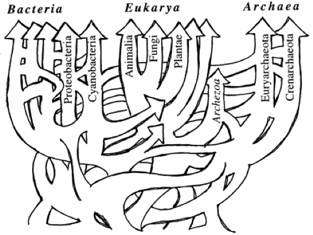
\includegraphics[width=.8\columnwidth]{./fig/introduction/doolittle_tree.png}
\caption[Ford Doolittle's Tree]{W Ford Doolittle's representation of the universal tree of life with nonvertical evolution. (From \emph{Science}, vol. 284, issue 5423, page 2127. Reprinted with permission from AAAS.)}
\label{fig:doolittle_tree}
\end{figure}

\section{Evolution as a Topological Space}

In this thesis, we propose the use of new computational techniques, borrowed from the field of algebraic topology, to capture and represent complex patterns of nonvertical evolution.
While this may sound obscure, let us unpack the basic idea.

Topology as a field is concerned with properties of spaces that are invariant under continous deformation.
Algebraic topology quantifies notions of shape by associating groups to invariants.
These invariants can include things such as connected components and holes in a topological space.
As a paradigmatic example, consider the coffee mug and donut (Figure~\ref{intro:fig:topology_example}.
The coffee mug can be continuously deformed into a donut without tearing.

Consider again Darwin's branching phylogeny (Figure~\ref{fig:darwin_origin}) and Doolittle's modified tree accounting for nonvertical processes (Figure~\ref{fig:doolittle_tree}).
The tree is trivially contractible and has relatively simple topology.
In contrast, Doolittle's construction has holes and is not contractible.
Here the topology is be much more complex.
However, we can adopt a similar perspective to the coffee mug example and characterize this space using homology.

To give the very simplest example, consider Figure~XX.
On the left we have a simple rooted three leaf evolutionary topology.
The topology is trivially contractible, which is captured by it's vanishing betti numbers above $d=1$.
On the right, we have a reticulate topology again involving three leaves.
Here, we can envision the center leaf as being a reticulation of genetic parents that are ancestral to the left and right leaves.
Betti numbers capture this.

Obviously there are complications that arise from, this but that is the basic idea.
First, deep evolutionary history consists of extinct organisms.
Second, we do not have complete sampling.
Third, not all organisms have compatible gene sets to make comparisons.
This is of course why Woese focused on conserved ribosomal RNA, some of the oldest genomic information.

\begin{figure}
\centering
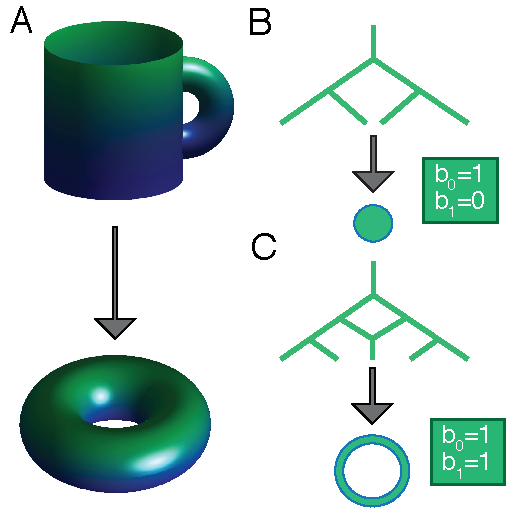
\includegraphics[width=.5\columnwidth]{./fig/introduction/topology_example.pdf}
\caption[The Paradigmatic Topology Example]{The coffee cup is not trivially contractible. The tree is contractible. The network is not contractible. Betti numbers quantitatively capture these notuons of shape.}
\label{intro:fig:topology_example}
\end{figure}

In this thesis, we use new computational techniques, borrowed from the field of algebraic topology, to capture and represent complex patterns of gene exchange that are obscurbed in current phylogenetic methods.
By doing so, we provide a fuller understanding of evolutionary relationships than allowed by current phylogenetic methods.
Genomic exchange can be characterized by the parental sequences involved in the exchange, by the amount and identity of material exchanged (i.e., the genes or loci involved), and the frequency with which similar exchanges occur.
Techniques such as phylogenetic networks and ancestral recombination graphs have been developed to describe reticulate evolution, but they have had only limited success due to difficulties of biological interpretation and computational infeasibility in all but the smallest datasets.

Linkage-based techniques have succeeded in measuring rates of recombination in medium-sized datasets (< 200 sequences), but they cannot reveal the scale of these exchanges (i.e., the genetic distance between parental sequences), and they have limited resolution in pinpointing where along a genome such exchanges have occurred.
A new mathematical foundation is needed to break free of these limitations.
Genome evolution is an extremely rich subject [cite Genome Architecture book].

This thesis contains results of applying methods from topological data analysis to various problems in genomics and evolution.
It primarily details the use of persistent homology as a tool to measure the prevalence and scale of nonvertical evolutionary events, such as reassortments and recombinations.
In so doing, various techniques are developed to extract statistical information from the topological complexes that are constructed.

\section{Thesis Organization}

The remainder of this thesis is organized as follows.

In Chapter \ref{ch:background} we present background information on the wide range of topics discussed in this thesis.
This discussion is chiefly structured into two pieces: (1) background on phylogenetics and population genetics, and (2) background on algebraic topology and the methods of topological data analysis.

In Part \ref{part:theory}, we develop two complementary approaches for analyzing genomic data using topological data analysis.
In Chapter \ref{ch:parametric_inference}, we develop methods for performing statistical inference using summary statistics contained in the persistence diagram.
This is the first such use of persistence diagrams as a tool for performing parametric inference.
In Chapter \ref{ch:complex_construction}, we propose alternative methods of constructing topological complexes that generalize the traditional Vietoris-Rips and \Cech complexes but are suited to the particular demands of phylogenetic applications.
We draw on previous work in phylogenetic networks and use homology theory to provide quantitative assessment of reticulation.

In Part \ref{part:application_microorganism} we apply our approach various microorganism datasets.
In Chapter \ref{ch:phage} we study bacteriophages.
In Chapter \ref{ch:influenza} we study influenza.
In Chapter \ref{ch:pathogens} we study pathogenic bacteria and use topological techniques to represent the spread of antibiotic resistance.
In Chapter \ref{ch:prokaryotes} we study prokaryotes.

In Part \ref{part:applications_human}, we apply our approaches to a several problems in human population genetics and biology.
In Chapter \ref{ch:human_recombination_rate} we measure the human recombination rate.
In Chapter \ref{ch:human_population_structre} we reconstruct models of human demographic movements.
In Chapter \ref{ch:human_chromatin_folding} we analyze Hi-C data to understand patterns of chromatin folding in the nucleus.
\kje{[May not be included; possibly an appendix section of virus results: flu, ebola, etc.]}

Finally, in Chapter \ref{ch:conclusions} we summarize our results and present possible avenues for future directions.